\documentclass[12pt, twoside]{article}
\usepackage[francais]{babel}
\usepackage[T1]{fontenc}
\usepackage[latin1]{inputenc}
\usepackage[left=5mm, right=5mm, top=5mm, bottom=3mm]{geometry}
\usepackage{float}
\usepackage{graphicx}
\usepackage{array}
\usepackage{multirow}
\usepackage{amsmath,amssymb,mathrsfs}
\usepackage{textcomp}
\pagestyle{empty}
\usepackage{soul}
\usepackage{eurosym}


\begin{document} 

%5e2 sujet 1

\begin{flushleft}
NOM PRENOM: \ldots \ldots \ldots \ldots \ldots \ldots \ldots \ldots \ldots
 \end{flushleft}


\begin{center}
{\fbox{$5^{e}2$ \qquad \qquad \textbf{\Large{Devoir surveill� 4 (sujet 1)}}
\qquad \qquad 15/03/2010}}
\end{center}

\bigskip


\textit{Remarque: L'exercice 3 et 5 sont � faire sur la photocopie, tous les
autres seront faits sur votre copie.}


\bigskip 
 


\ul{\textbf{Exercice 1:}} \textit{(3 points)} 

\begin{enumerate}
  
  \item Construire le triangle KLM tel que KL=7cm, KM=4,5cm et ML=6cm.
  \item Construire le triangle RST tel que $\widehat{RST}$=43�, ST=5cm et
  $\widehat{RTS}$=100�.
\end{enumerate}


\bigskip

\medskip


\ul{\textbf{Exercice 2:}} \textit{(4 points)}


\begin{enumerate}
\item Reproduire la figure ci-dessous en vraie grandeur.
\item R�diger un programme de construction.
\end{enumerate}

\begin{center}
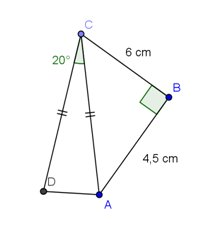
\includegraphics[width=4cm]{images/pgm-construction.jpg}
\end{center}

\bigskip

\medskip


\ul{\textbf{Exercice 3:}} \textit{(3 points)} 


\begin{enumerate}
\item Le triangle AEI tel que AI=5mm; AE=7mm et EI=1,5mm existe-t-il? Justifier
votre r�ponse.

\item  Le triangle IJK tel que IJ=10,1m; IK=5,6m et KJ=4,8m existe-t-il?
Justifier votre r�ponse.
\end{enumerate}

\bigskip

\medskip

\ul{\textbf{Exercice 4:}} \textit{(2 points)} 


\begin{enumerate}
  \item On sait que AB=3cm; AC=7cm et BC=4cm. Entoure sur cette feuille la
  bonne r�ponse:
  
  
  \begin{center}
  $B \in [AC]$ \qquad \qquad \qquad \qquad $A \in [BC]$ \qquad \qquad \qquad
  \qquad $C \in [AB]$
  \end{center}


  \item R, S et T sont trois points tels que RS=11cm; RT=2cm et $T \in [RS]$.
  Entoure sur cette feuille la bonne r�ponse:
  
  
  \begin{center}
  TS=21cm \qquad \qquad \qquad \qquad TS=9cm \qquad \qquad \qquad \qquad TS=13cm
  \end{center}
\end{enumerate}



\bigskip

\medskip


\ul{\textbf{Exercice 5:}} \textit{(5 points)}

\begin{enumerate}
  \item Quelle est la propri�t� des angles d'un triangle? \ldots \ldots \ldots
  \ldots \ldots \ldots \ldots \ldots \ldots \ldots \ldots \ldots \ldots \ldots
  \ldots \ldots \ldots \ldots \ldots 

\item 
Compl�ter le tableau suivant:
\begin{center}
\begin{tabular}{|c|c|c|c|c|c|}
\hline

\qquad \qquad & ABC est & ABC est  & ABC est & ABC est & ABC est \\
\qquad \qquad & quelconque & isoc�le en B & rectangle en C & \ldots \ldots
\ldots \ldots \ldots \ldots \ldots \ldots & \ldots \ldots \ldots \ldots \ldots
\ldots \ldots \ldots \\

\hline

$\widehat{A}$ & 65� & \ldots \ldots & 30� & 32� & 45� \\
\hline

$\widehat{B}$ & 37� & \ldots \ldots & \ldots \ldots & 116� & \ldots \ldots \\

\hline

$\widehat{C}$ & \ldots \ldots & 75� & \ldots \ldots & \ldots \ldots & 45� \\
\hline
\end{tabular}
\end{center}
\end{enumerate}

\bigskip

\bigskip
 

\ul{\textbf{Exercice 6:}} \textit{(3 points)}

\begin{enumerate}
  \item Calculer la mesure de l'angle $\widehat{ABE}$. Justifier votre r�ponse.
  \item Calculer la mesure de l'angle $\widehat{DBC}$. Justifier votre r�ponse.
  \item Les points A, B et C sont-ils align�s? Justifier votre r�ponse.
\end{enumerate}

\pagebreak

%5e2 sujet 2

\begin{flushleft}
NOM PRENOM: \ldots \ldots \ldots \ldots \ldots \ldots \ldots \ldots \ldots
 \end{flushleft}


\begin{center}
{\fbox{$5^{e}2$ \qquad \qquad \textbf{\Large{Devoir surveill� 4 (sujet 2)}}
\qquad \qquad 15/03/2010}}
\end{center}

\bigskip


\textit{Remarque: L'exercice 3 et 5 sont � faire sur la photocopie, tous les
autres seront faits sur votre copie.}


\bigskip 
 


\ul{\textbf{Exercice 1:}} \textit{(3 points)} 

\begin{enumerate}
  
  \item Construire le triangle RST tel que RS=7cm, ST=4,5cm et TR=6cm.
  \item Construire le triangle KLM tel que $\widehat{KLM}$=43�, LK=5cm et
  $\widehat{MKL}$=100�.
\end{enumerate}


\bigskip

\medskip


\ul{\textbf{Exercice 2:}} \textit{(4 points)}


\begin{enumerate}
\item Reproduire la figure ci-dessous en vraie grandeur.
\item R�diger un programme de construction.
\end{enumerate}

\begin{center}
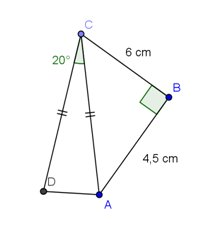
\includegraphics[width=4cm]{images/pgm-construction.jpg}
\end{center}

\bigskip

\medskip


\ul{\textbf{Exercice 3:}} \textit{(3 points)} 


\begin{enumerate}
\item Le triangle AEI tel que AE=5,5mm; AI=7mm et EI=1mm existe-t-il?
Justifier votre r�ponse.

\item  Le triangle IJK tel que IJ=10,2m; JK=5,6m et KI=4,7m existe-t-il?
Justifier votre r�ponse.
\end{enumerate}

\bigskip

\medskip

\ul{\textbf{Exercice 4:}} \textit{(2 points)} 


\begin{enumerate}
  \item On sait que AC=3cm; CB=7cm et B=4cm. Entoure sur cette feuille la
  bonne r�ponse:
  
  
  \begin{center}
  $B \in [AC]$ \qquad \qquad \qquad \qquad $A \in [BC]$ \qquad \qquad \qquad
  \qquad $C \in [AB]$
  \end{center}


  \item O, U et I sont trois points tels que UO=11cm; UI=2cm et $I \in [UO]$.
  Entoure sur cette feuille la bonne r�ponse:
  
  
  \begin{center}
  IO=21cm \qquad \qquad \qquad \qquad IO=9cm \qquad \qquad \qquad \qquad IO=13cm
  \end{center}
\end{enumerate}



\bigskip

\medskip


\ul{\textbf{Exercice 5:}} \textit{(5 points)}

\begin{enumerate}
  \item Quelle est la propri�t� des angles d'un triangle? \ldots \ldots \ldots
  \ldots \ldots \ldots \ldots \ldots \ldots \ldots \ldots \ldots \ldots \ldots
  \ldots \ldots \ldots \ldots \ldots 

\item 
Compl�ter le tableau suivant:
\begin{center}
\begin{tabular}{|c|c|c|c|c|c|}
\hline

\qquad \qquad & ABC est & ABC est  & ABC est & ABC est & ABC est \\
\qquad \qquad & quelconque & isoc�le en B & rectangle en C & \ldots \ldots
\ldots \ldots \ldots \ldots \ldots \ldots & \ldots \ldots \ldots \ldots \ldots
\ldots \ldots \ldots \\

\hline

$\widehat{A}$ & 75� & \ldots \ldots &60� & 34� & 45� \\
\hline

$\widehat{B}$ & 38� & \ldots \ldots & \ldots \ldots & 112� & \ldots \ldots \\

\hline

$\widehat{C}$ & \ldots \ldots & 85� & \ldots \ldots & \ldots \ldots & 45� \\
\hline
\end{tabular}
\end{center}
\end{enumerate}

\bigskip

\bigskip
 

\ul{\textbf{Exercice 6:}} \textit{(3 points)}

\begin{enumerate}
  \item Calculer la mesure de l'angle $\widehat{ABE}$. Justifier votre r�ponse.
  \item Calculer la mesure de l'angle $\widehat{DBC}$. Justifier votre r�ponse.
  \item Les points A, B et C sont-ils align�s? Justifier votre r�ponse.
\end{enumerate}
\end{document}
